
%Because it includes an on-shell Z boson as well as a b-jet and W from the top decay, tZ production represents an identical final state  to WZ + b-jet. This implies the possibility of matrix level interference between these two processes not accounted for in the Monte Carlo simulations, which consider the two processes independently. Truth level studies are performed in order to estimate the impact of these interference effects.

An important process to consider in this analysis is tZ: the top almost always decays into a W boson and b-quark, and when both the W and Z decay leptonically, this gives three leptons and a heavy flavor jet in the final state. Because tZ can produce a final state identical to the signal, it represents a predominant background in the most signal enriched regions. That is, the region with one jet passing the 60\% DL1r WP. Therefore, a boosted decision tree (BDT) algorithm is trained using XGBoost \cite{xgboost_cite} to separate $WZ$ + heavy flavor from tZ. The result of this BDT is used to create a tZ enriched region in the fit, reducing its impact on the measurement of WZ + heavy flavor.

The following kinematic variables are used as inputs to train this BDT:
 
\begin{itemize}
     \item The invariant mass of the reconstructed top candidate
     \item $p_T$ of each of the leptons, jet
     \item The  invariant mass of each combination of lepton pairs, $M(ll)$
     \item $E_T^{miss}$
     \item Distance between each combination of leptons, $\Delta R (ll)$
     \item Distance between each lepton and the jet, $\Delta R (lj)$
\end{itemize}


Here the top candidate is reconstructed based on the procedure described in section 6.1 of \cite{ttZ_paper}. Broadly, the mass of the top quark candidate is reconstructed from the jet, the lepton not included in the Z-candidate, and a reconstructed neutrino. In the case that there is one jet in the event, there is only possible b-jet candidate. For events with two jets, the jet with the highest DL1r score is used.
 
The training samples included only events meeting the requirements of the 1-jet, >60\% region, i.e. passing all the selection described in section \ref{sec:evt_selection} and having exactly one jet which passes the tightest (60\%) DL1r working point.A sample of 20,000 background (tZ) and signal (WZ+b) Monte Carlo events are used to train the BDT. And additional 5,000 events are reserved for testing the model, in order to prevent over-fitting. A total of 750 decision trees with a maximum depth of 6 branches are used to build the model. These parameters are chosen empirically, by training several models with different parameters and selecting the one that gave the best separation for the test sample. 

The results of the BDT training are shown in figure \ref{fig:tZ_bdt}. The output scores for both signal and background events is shown on the left. The right shows the receiving operating characteristic (ROC) curve that results from the MVA. The ROC curve represents the background rejection as a function of signal efficiency, where each point on the curve represents a different response score. The ROC curve of the BDT is compared to the performance of using an optimal set of flat selections on the same set of input variables.

\begin{figure}[H] 
\center
    \subfigure[]{\includegraphics[width=.45\linewidth]{tZ_bdt_ab127/plots_nlo/xgb_score.png}}%
    \subfigure[]{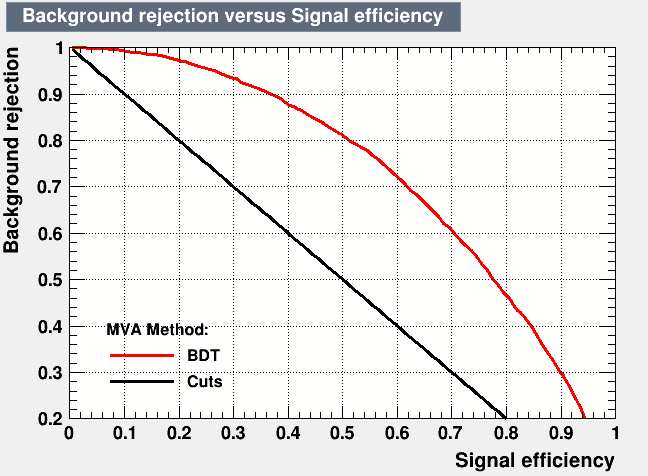
\includegraphics[width=.45\linewidth]{tZ_bdt_ab127/plots_nlo/roc.png}}    
    \caption{Distribution of the BDT response for signal and background events on the left, the ROC curve for the BDT on the right.}
    \label{fig:tZ_bdt}
\end{figure}

The relative important of each input feature in the model, measured by how often they appeared in the decision trees, is shown in figure \ref{fig:tZ_fImp}.

\begin{figure}[H] 
\center
        \includegraphics[width=0.9\linewidth]{tZ_bdt/feature_importance.png}
        \caption{Relative importance of each input feature in the model.}
        \label{fig:tZ_fImp}
\end{figure}

These results suggest that some amount of separation can be achieved between these two processes, with a high BDT score selecting a set of events that is pure in $WZ$ + b. A BDT score of 0.725 is selected as a cutoff, where events with scores higher than this form a signal enriched region, and events with scores lower than this form a tZ control region. This cutoff is selected by varying the value of thia cutoff in stat-only Asimov fits, and selecting the value that minimizes the statistical uncertainty on WZ + b.

